\section{Correctness Checks}
\label{app:acceptance}

The protocol applies to functions whose effects are expressed inside Lean, including pure functions and computations in monads such as \texttt{Id}, \texttt{StateM}, and \texttt{Except}, and excludes functions whose behavior depends on opaque effects such as \texttt{IO} or foreign calls.
For these functions, the equality theorem covers every input without a bound on input size or recursion depth.
Following Vero~\citep{ye2026vero}, the acceptance checker extracts the submitted declarations and inserts them into a fresh copy of the reference environment.
It then applies four checks to protect the reference, validate the proof, and ensure that the executable replacement is the definition being proved.
\begin{enumerate}[leftmargin=*]
\item \textbf{Build.} In the fresh environment, every existing declaration of $\mathcal{R}$, including the reference $f$ and its callers, remains byte-identical, and the submission adds only the replacement $f'$, its auxiliary definitions and lemmas, and the proof $\pi$. In a separate integration check, the acceptance checker registers the equality theorem as a \texttt{@[csimp]} replacement, so compiled callers use $f'$, and checks that the resulting repository $\mathcal{R}'$ builds with all submitted declarations.
\item \textbf{Axioms.} The axioms used by $\pi$ and every auxiliary declaration, including through their dependencies, must be a subset of $\{\texttt{propext}, \texttt{Quot.sound}, \texttt{Classical.choice}\}$. In particular, \texttt{sorryAx} is forbidden.
\item \textbf{Executability.} The rewrite and its agent-supplied computational dependencies must be computable, without \texttt{partial} or \texttt{unsafe} definitions or \texttt{@[implemented\_by]} and \texttt{@[extern]} substitutions. They use the fixed library and runtime supplied with the task.
\item \textbf{Kernel-only checking.} The proof must not use \texttt{native\_decide}, which appeals to compiled execution to discharge a proof step.
\end{enumerate}
Condition 3 prevents executable substitutions for the definition being proved, while Condition 4 requires proof steps to be checked by the kernel.
The protocol also rejects agent-introduced typeclass instances that would change the interpretation of equality for the types involved.
The checked proof and its dependencies can be replayed in Lean.
Accepted implementations are compiled and timed with the task's fixed Lean compiler, standard library, and runtime.


\section{Migration Pipeline and Results}
\label{app:migration}

\paragraph{Pipeline.}
The migration workflow produces the Lean references used by the optimizer.
Its three candidate strategies emphasize broad interface coverage, executable fixtures, and an explicit ledger of behavioral obligations.
Separate test-design agents inspect frozen candidates and generate inputs for uncovered behavior, boundary cases, and disagreements between ports.
The controller compares each port with the original on those inputs, selects a candidate, and coordinates repair.
Coverage and mutation feedback guide further test generation.
Migration runs in the benchmark's white-box setting.
Agents may read the pinned source and execute the original program, but the hidden tests and any signal derived from them stay inaccessible throughout, so the scores measure generalization to behavior that no agent observed.
We compare \aqueduct{} against a baseline of one migration agent given the source repository and the migration task, which represents what one-shot agentic migration achieves without the pipeline.
Both run in the same setting with the same model.

\paragraph{Interface comparison.}
The same comparison rule applies to the generated corpus $T$ during migration and to $T_{\mathrm{hidden}}$ at the final evaluation.
Unstable behavior, including randomness, host-dependent floating-point formatting, and language-specific error text, is excluded from that interface or handled by its declared comparison rule.
Applying the same comparison rule throughout candidate selection, repair, and hidden evaluation keeps the required behavior consistent across the migration process.

\paragraph{Recovery.}
ProgramBench declares 39,857 tests across the 40 sampled repositories, of which the original programs pass 18,642 in the evaluation environment.
Recovery is the fraction of these original-supported tests that the port passes.
Across these repositories, the \aqueduct{} ports pass 16,345 tests and the single-agent baseline passes 12,709, or 87.68\% and 68.17\% recovery.

\paragraph{Generated-test quality.}
The pipeline rests on the premise that generated evidence must discriminate, telling faithful ports apart from unfaithful ones and exposing the faults a weaker suite would miss.
We evaluate this premise directly with mutation analysis.
After the test suites are frozen, we inject deterministic source-level faults into the original programs, rebuild each mutated checkout, and count only mutants that compile.
A mutant is killed only when a test that passes on the unmutated program fails on the mutant.
Because the faults are planted after freezing, the audit is independent of the migration search that produced the tests.
The test-design agents generated 33,671 behavioral tests across the 40 migration targets.

\emph{Generated tests versus the benchmark's own tests.}
The central question is whether the generated suite observes behavioral differences that the external benchmark does not, so we score the same compiled mutants under both the generated tests and the hidden ProgramBench tests.
On 36 compiled mutants across 9 repositories, the generated tests kill 28 (77.8\%) against 17 (47.2\%) for ProgramBench (Table~\ref{tab:mutants}).
The asymmetry is sharpest among mutants that exactly one suite catches.
The generated tests account for 12 of these 13, ProgramBench for 1 (exact paired binomial $p = 0.0034$).
The generated suite discriminates behavioral differences that the benchmark's own tests do not observe, which is why the pipeline generates its evidence rather than borrowing it.

\begin{table}[h]
\centering
\caption{Mutants killed by the generated tests and by the hidden ProgramBench tests on the same 36 compiled mutants across 9 repositories.}
\label{tab:mutants}
\small
\begin{tabular}{lr}
\toprule
Outcome & Mutants \\
\midrule
Killed by both suites & 16 \\
Killed by generated tests only & 12 \\
Killed by ProgramBench tests only & 1 \\
Killed by neither & 7 \\
\midrule
Total scored & 36 \\
\bottomrule
\end{tabular}
\end{table}

\emph{Auditing the suite against itself.}
We also measure the generated suite's absolute kill rate on the full audit population (Table~\ref{tab:mutation-audit}).
The 95\% interval is a repository-cluster bootstrap.
These are end-to-end behavioral tests at the program boundary, where a source-level mutant registers only if its effect propagates to observable output, so interface-level kill rates run below what unit-level mutation testing reports.
Within the pipeline, each surviving mutant marks a behavior that the corpus executes but does not yet constrain, and it becomes a target for the next round of test generation.
The behaviors the suite does not yet check are therefore enumerated, as in the 7zip case study, which itemizes the port's remaining obligations.

\begin{table}[h]
\centering
\caption{Mutation audit of the generated suite on the full audit population.}
\label{tab:mutation-audit}
\small
\begin{tabular}{rrrrrr}
\toprule
Repositories & Compiled mutants & Killed & Score & Median per repository & 95\% interval \\
\midrule
25 & 190 & 101 & 53.2\% & 50.0\% & 39.1\% to 67.0\% \\
\bottomrule
\end{tabular}
\end{table}

\section{Migration Ablations}
\label{app:ablation}

Figure~\ref{fig:migration-ablations} compares the full pipeline with four component ablations and two baselines.
\emph{One repair round.} The pipeline runs candidate generation, test design, and selection in full, but performs a single round of repair instead of alternating repair with evidence generation until convergence. This measures the full repair loop.
\emph{No coverage guidance in the testing loop.} The testing loop loses coverage instrumentation, so test generation no longer learns which code paths remain unexercised. This measures the coverage signal.
\emph{No mutation feedback in the testing loop.} The testing loop loses mutation testing, so faults the corpus fails to catch no longer become targets for the next round of test generation. This measures the mutation signal.
\emph{No candidate portfolio (best single strategy).} A single migration agent ports each package under one fixed strategy instead of three. We run each of the three strategies this way and the figure reports the best one. This measures candidate diversity and selection together.
\emph{Baseline (single agent, no pipeline).} A plain agent ports each package.
\emph{Fixed phased pipeline.} A variant with the same migration and testing tools exposes them as a fixed sequence of phases. This measures the value of letting agents revisit earlier steps rather than follow a fixed order.

\paragraph{Each component contributes to recovery.}
The full pipeline recovers 87.68\% of the original behavior against 68.17\% for a single agent with the same source and toolchain, and every component ablation falls between the two, while the fixed phased pipeline falls below the single agent.
The following paragraphs attribute this gap to individual components.

\paragraph{Iterative repair outperforms a fixed sequence of phases.}
The phased pipeline recovers less than even the single-agent baseline, and it contains the same tools as the full pipeline, so the tools are not the bottleneck.
Its phases run in a fixed order and never revisit earlier decisions, so when a later phase uncovers behavior the port misses, the agent cannot return to update the behavioral surface it committed to earlier.
The agents fill gaps in their ports when they can revisit earlier decisions, but not when a fixed sequence prevents it.
This result suggests giving agents freedom over how they work and concentrating rigor in the acceptance criteria and the checks that judge the result.

\paragraph{Candidate diversity provides the largest gain.}
Committing to the best single migration strategy caps recovery at 72.96\%.
The controller picks the first strategy for 18 repositories, the second for 20, and the third for 2, so no strategy dominates and the gain comes from having a portfolio and the evidence to choose among it.
This also reflects a structural property of the search.
Repair is incremental and rarely changes a port's overall structure, so the structural diversity that matters must already exist among the initial candidates.

\paragraph{Both testing signals improve the corpus in complementary ways.}
Removing coverage guidance or mutation feedback costs 9.80 and 10.05 points, more than the 8.46 points lost by restricting repair to a single round, so the quality of the test corpus matters more than the repair loop that consumes it.
The two signals match their designed roles.
Coverage guidance steers test generation toward behavior no test has exercised, and mutation feedback hardens the checks on behavior the corpus already reaches.
Repair can only fix what a test exposes, so a weaker corpus leaves divergences undetected and the pipeline treats them as agreement.

\begin{figure}[t]
\centering
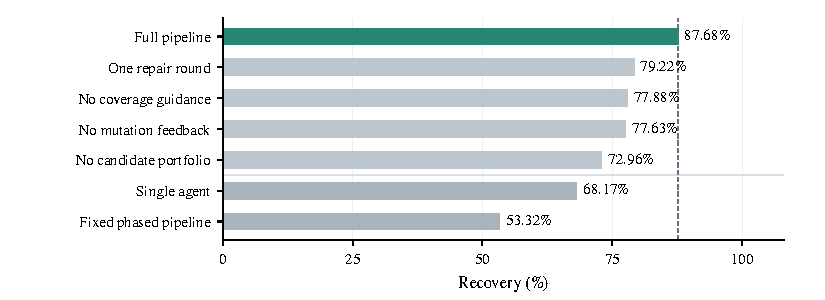
\includegraphics[width=\linewidth]{figures/paper/migration-ablations.pdf}
\caption{\textbf{Contribution of migration components.} Recovery under component ablations and two pipeline baselines. Removing candidate diversity produces the largest decrease among the four component ablations.}
\label{fig:migration-ablations}
\end{figure}

\section{Additional Case Studies}
\label{app:casestudies}

\subsection{Longest Increasing Subsequence}
\label{app:lis-proof}

The following theorem and proof establish equivalence for the rewrite in Figure~\ref{fig:task-format}.
The input \code{nums} is an arbitrary list of integers, so the theorem covers every such list.
The proof quantifies over \code{prev}, the optional preceding element used by the recursive helper, and shows that querying the computed table returns the same length as that helper.

\noindent\begin{minipage}{\linewidth}
\lstinputlisting[language=lean,firstline=72,lastline=102,firstnumber=1]{examples/verina_advanced_33.lean}
\end{minipage}

Across the 261 inputs in the evaluation corpus, median time per corpus pass falls from $1.424$ seconds to $318.653$ microseconds, a speedup of $4{,}467.871\times$.

\subsection{Migration at Scale: 7zip}

7zip is the fourth largest repository in our sample at 252,968 lines of source, and it tests whether the pipeline can expand a port across a large behavioral surface for frequently used real-world software.
ProgramBench declares 883 original-supported tests for 7zip, spanning more than a dozen archive formats and their command-line, stream, and filesystem interactions.
The final port recovers 554 of them (62.74\%), against 28.77\% for the baseline, a direct measure of where migration is hardest.
The port is a substantial native Lean implementation.
It handles ZIP, TAR, 7z, bzip2, Zstandard, raw LZMA and LZMA86, split archives, AR and DEB, CPIO, RPM, ISO-9660 with Joliet, and CAB with None and MSZip compression, and it implements listing, testing, extraction, creation, update and delete paths, include and exclude filters, standard-stream routing, overwrite behavior, and hash manifests.
No single porting attempt produces this surface.
It accumulates through the search, as test-design agents surface unhandled formats and options, each divergence becomes a repair target, and each repaired behavior freezes into a permanent regression case.
At the final checkpoint the port passes 541 of 579 generated behavioral tests, and the search's inventory of behavioral obligations still lists 938 open items when the budget is exhausted, behaviors the corpus has named but not yet established evidence for.
These open obligations account for the gap between the generated-corpus pass rate and hidden-set recovery.
The port's remaining gaps are thus measured and itemized, and they direct the next round of the search.

\subsection{Optimization Case Studies}

We examine five proved optimizations that illustrate the three rewrite patterns of Section~\ref{sec:eval-aqueduct}.

\paragraph{Algorithmic improvement (Cheat \texttt{findConsolidated}).}
The migrated function first builds the complete consolidated sheet list and then searches it for the requested title, so every lookup pays for constructing entries it immediately discards.
The optimized declaration searches from the end of the ordered paths and returns the last matching title directly, never materializing the intermediate list.
The equality theorem proves that direct reverse search returns exactly the element the build-then-search pipeline would find, folding the consolidation semantics into the lookup.
The migrated declaration is already faster than the matched Go operation, and the rewrite, $5.46\times$ faster than migrated Lean, widens that margin to $20.36\times$ by removing the build-then-search work that the Go code also performs.

\paragraph{Algorithmic improvement (Cheat \texttt{consolidatedSheets}).}
The migrated function builds its result by filtering the entire accumulated list before every append, repeatedly traversing and reallocating a growing structure.
The optimized declaration walks the input once in reverse, tracks seen titles in a hash set, and constructs the output list once.
The equality theorem proves that the reverse traversal preserves the exact last-title-wins semantics of the original fold, a property that is easy to get wrong in a manual rewrite.
The rewrite is $1.46\times$ faster than migrated Lean and $6.65\times$ faster than the matched Go operation.

\paragraph{Representation improvement (Gron \texttt{validIdentifier}).}
The migrated function materializes a full character list to check an identifier.
The optimized declaration reads the first character directly and checks the remainder through a string slice, allocating nothing.
The theorem composes the slice-to-list equivalence with previously proved character-classification replacements, so later proofs reuse lemmas from earlier rewrites.
The rewrite is $1.96\times$ faster than migrated Lean and $2.10\times$ faster than Go.

\paragraph{Algorithmic improvement (Cheat \texttt{filterSheets}).}
The migrated function re-trims every requested tag once per sheet.
The optimized declaration normalizes the tags once and reuses the prepared list across all sheets, changing repeated normalization into a single pass.
The rewrite is $5.45\times$ faster than migrated Lean and $2.01\times$ faster than the matched Go operation, and the output checksums agree across all three implementations.

\paragraph{Evaluation-order improvement (Code Minimap \texttt{pow10}).}
The migrated helper enters its multiplication loop even for a zero exponent.
The optimized declaration returns the zero case immediately, producing a $9.29\times$ within-Lean speedup and running $1.37\times$ faster than the Rust original on a microbenchmark whose inputs include the zero exponent.
The equality theorem shows that the fast path changes no result, because the declarations with and without the fast path are equal on every input.
Under the equivalence obligation, the agent can therefore add fast paths for inputs it expects to be common without restricting correctness to those inputs.

In all five cases, the rewrite removes a pattern common in migrated code, such as repeated filtering, intermediate materialization, redundant normalization, or a missed fast path, and the equality proof guarantees that removing the pattern preserves behavior on every input.
